\chapter{Micro-Stressing Benchmarks}
\label{cha:micro-benchs}
This chapter presents strategies relying on benchmarks to figure out the
characteristics of an architecture, be it its speed, the capacity of its
components, or other information not sufficiently detailed in the architecture's
documentation. Having properly characterized the architecture is a
necessary preliminary step to the analysis of interference. Indeed, to
understand the effects the interference has on running software, a
quantification of the architecture's components capabilities is necessary, as
determining which parallel accesses would interfere with one another is
otherwise impossible.

In the contributions made by this thesis, the objective of the benchmarks is not
only to measure the maximum performance of the cache coherence mechanisms, but
also ascertain that they are fully understood by the user. This is a vital part
of the characterization process, and solutions for mechanisms much simpler than
cache coherence have already been explored. For example, the first section of
this chapter showcases two papers proposing solutions to detect hidden
correlations between components.

Once the mechanisms have been understood, then the performance measurements can
proceed, as the user is now fully aware of what is being measured. The second
section of this chapter is thus about papers on the use of benchmarks for the
performance analysis of cache coherence.

Lastly, this chapter presents a paper on the use of benchmarks to remedy a lack
of performance monitors. Such an approach could be used to implement the
solution proposed in Chapter~\ref{cha:identifying_cache_coherence} if the user
cannot find the appropriate performance monitors.

Because the terms are recurrently used thorough this chapter, definitions for
\textit{execution time}, \textit{overhead}, and \textit{bandwidth} are provided below.

\begin{definition}[Configuration]
\label{def:configuration}
A configuration is defined as the combination of the mapping of programs on each
core, the hardware's settings, and the initial state of the architecture prior
to program execution.
\end{definition}

\begin{example}[Configuration]
\label{ex:configuration}
Running a sequence of instructions in isolation, and running that same sequence
of instructions while other programs are running on other cores correspond to
two separate configurations.
\end{example}

\begin{definition}[Execution Time]
The execution time of a list of instructions on a certain configuration is the
time between the emission of the first of the instructions and the last
instruction of the list being seen as completed by the emitter.
\end{definition}

\begin{example}[Execution Time]
In the case of two successive loads, the execution time corresponds to the time
elapsed between core emitting the first load instruction to its cache, and the
cache providing the data for the second load instruction.
\end{example}


\begin{definition}[Overhead]
Given $T_A$ and $T_B$ two execution times of a same list of instructions from
two separate arbitrary configurations $A$ and $B$, such that $T_B \ge T_A$, The
overhead $O$ of being in configuration $B$ over configuration $A$ is defined as:
\[ O = T_B - T_A \]
\end{definition}

\begin{example}[Overhead]
If the two configurations of Example~\ref{ex:configuration} yielded an execution
time of 5 CPU cycles and 13 CPU cycles respectively, the overhead incurred
because of the other programs running in parallel would be $13 - 5 = 8$ CPU
cycles.
\end{example}

\begin{definition}[Bandwidth]
Bandwidth is the amount of data (e.g.~bits, bytes, words) that can be
transferred from one component to another within a given time frame.
\end{definition}

\begin{example}[Bandwidth]
A CPU attempting to write a sequence of data with a size of 512MB in the memory
would have to pass the information through all the mechanisms between itself and
the memory. The amount of data that went through all the mechanisms within
either a CPU cycle or a microsecond is considered to be the bandwidth.
\end{example}

\stopallthesefloats{}
\section{Detecting Component Correlation}
\stopallthesefloats{}
\stopallthesefloats
\subsection{Evaluating Interference Through Resource-Stressing}
\label{sec:radojkovic}
\cite{10.1145/2086696.2086713} presents a strategy to characterize the
sensibility of a shared resource to temporal interference. The general idea
behind the approach is to perform a stressing benchmark on an architecture's
resource with only that single thread running (i.e.~running in isolation), and
compare the result with the same test in which multiple threads of the stressing
benchmark run in parallel, in a metric called \textit{slowdown factor} (see
Definition~\ref{def:slowdown-factor}).

\begin{definition}[Slowdown Factor]
\label{def:slowdown-factor}
Given a benchmark targeting a specific component, its application using a single
thread in isolation resulting in a execution time $n$, and its application while other
threads are stressing components (potentially the same one) yielding a execution time
of $m$, the slowdown factor $f$ is defined as:
\[f = \frac{n}{m}\]
\end{definition}

This slowdown factor indicates how sensible the component targeted by the
measured benchmark is to interference, and thus how large the execution time
variations caused by parallel access to that component will be. By having the
other threads target different components, correlation between them can be
exposed: if the slowdown factor is higher than $1.0$, some interactions occur
between these components, and the other components are able to generate
interference on any application using the component targeted by the measured
thread.
\begin{figure}[hbt!]
\begin{center}
%\lstinputlisting{\chapterdirectory/figure/micro_bench/atom_bench.txt}
\begin{tabular}{r|l|l}
\hline
Line  & Source code                    & Explanation\\
\hline
001   & {\lstinline!movl %1, %ecx!}    & initialize loop counter \textit{ecx}
({\lstinline!%1!} is an input parameter)\\
002   & {\lstinline!label_intAdd:!}    & beginning of the loop\\
003   & {\lstinline!add %eax, %ebx!}   & target instruction\\
004   & {\lstinline!add %ebx, %eax!}   & target instruction\\
...   & {\lstinline!...!}              & ...\\
...   & {\lstinline!...!}              & ...\\
252   & {\lstinline!add %ebx, %eax!}   & target instruction\\
253   & {\lstinline!decl %ecx!}        & decrement loop counter\\
254   & {\lstinline!cmp %ecx, $0!}     & compare loop counter with 0\\
255   & {\lstinline!jne label_intAdd!} & if (counter != 0) jump to the beginning of the loop\\
\hline
\end{tabular}
\end{center}
\caption{\textit{intAdd} Benchmarking Code (taken from
\cite{10.1145/2086696.2086713})}%
\label{fig:micro_bench:atom_bench}
\end{figure}

\begin{figure}[hbt!]
\begin{center}
\lstinputlisting{\chapterdirectory/figure/micro_bench/atom_init.txt}
\end{center}
\caption{Memory Benchmark Initialization Code (taken from
\cite{10.1145/2086696.2086713})}%
\label{fig:micro_bench:atom_init}
\end{figure}

The benchmarks of \cite{10.1145/2086696.2086713} are implemented following the
pattern shown in Figure~\ref{fig:micro_bench:atom_bench}: a simple loop applying
the appropriate instruction numerous times. For memory access benchmarking, a
slightly different strategy is used (see
Figure~\ref{fig:micro_bench:atom_init}): each loaded memory element contains the
address of the next memory element to load, a principle known as pointer
chasing.

\begin{figure}[hbt!]
\begin{center}
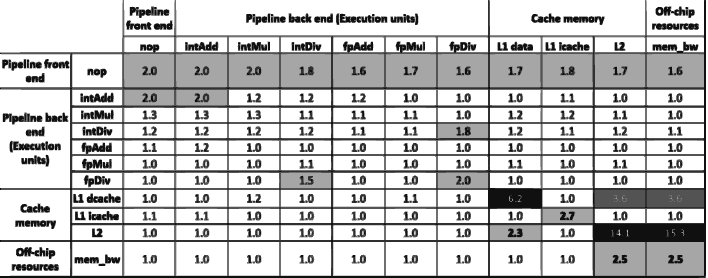
\includegraphics[width=\textwidth]{\chapterdirectory/figure/micro_bench/atom_stress.pdf}
\end{center}
\caption{Slowdown factor on the Intel Atom Z530 (taken from \cite{10.1145/2086696.2086713})}%
\label{fig:micro_bench:atom_stress}
\end{figure}

Figure~\ref{fig:micro_bench:atom_stress} shows the approach of
\cite{10.1145/2086696.2086713} working at its best. This is the result on an
Intel Atom Z530, which features a single core capable of running two parallel
threads. The lines correspond to the benchmark being measured, the columns
correspond to the target of the benchmark being used as a source of
interference.

\begin{figure}[hbt!]
\begin{center}
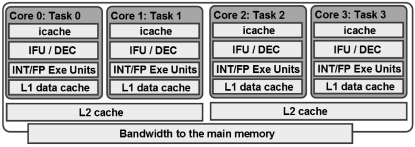
\includegraphics[width=0.6\textwidth]{\chapterdirectory/figure/micro_bench/core2quad.png}
\end{center}
\caption{The Intel Core2Quad architecture (taken
from \cite{10.1145/2086696.2086713})}%
\label{fig:micro_bench:core2quad}
\end{figure}

\begin{figure}[hbt!]
\begin{center}
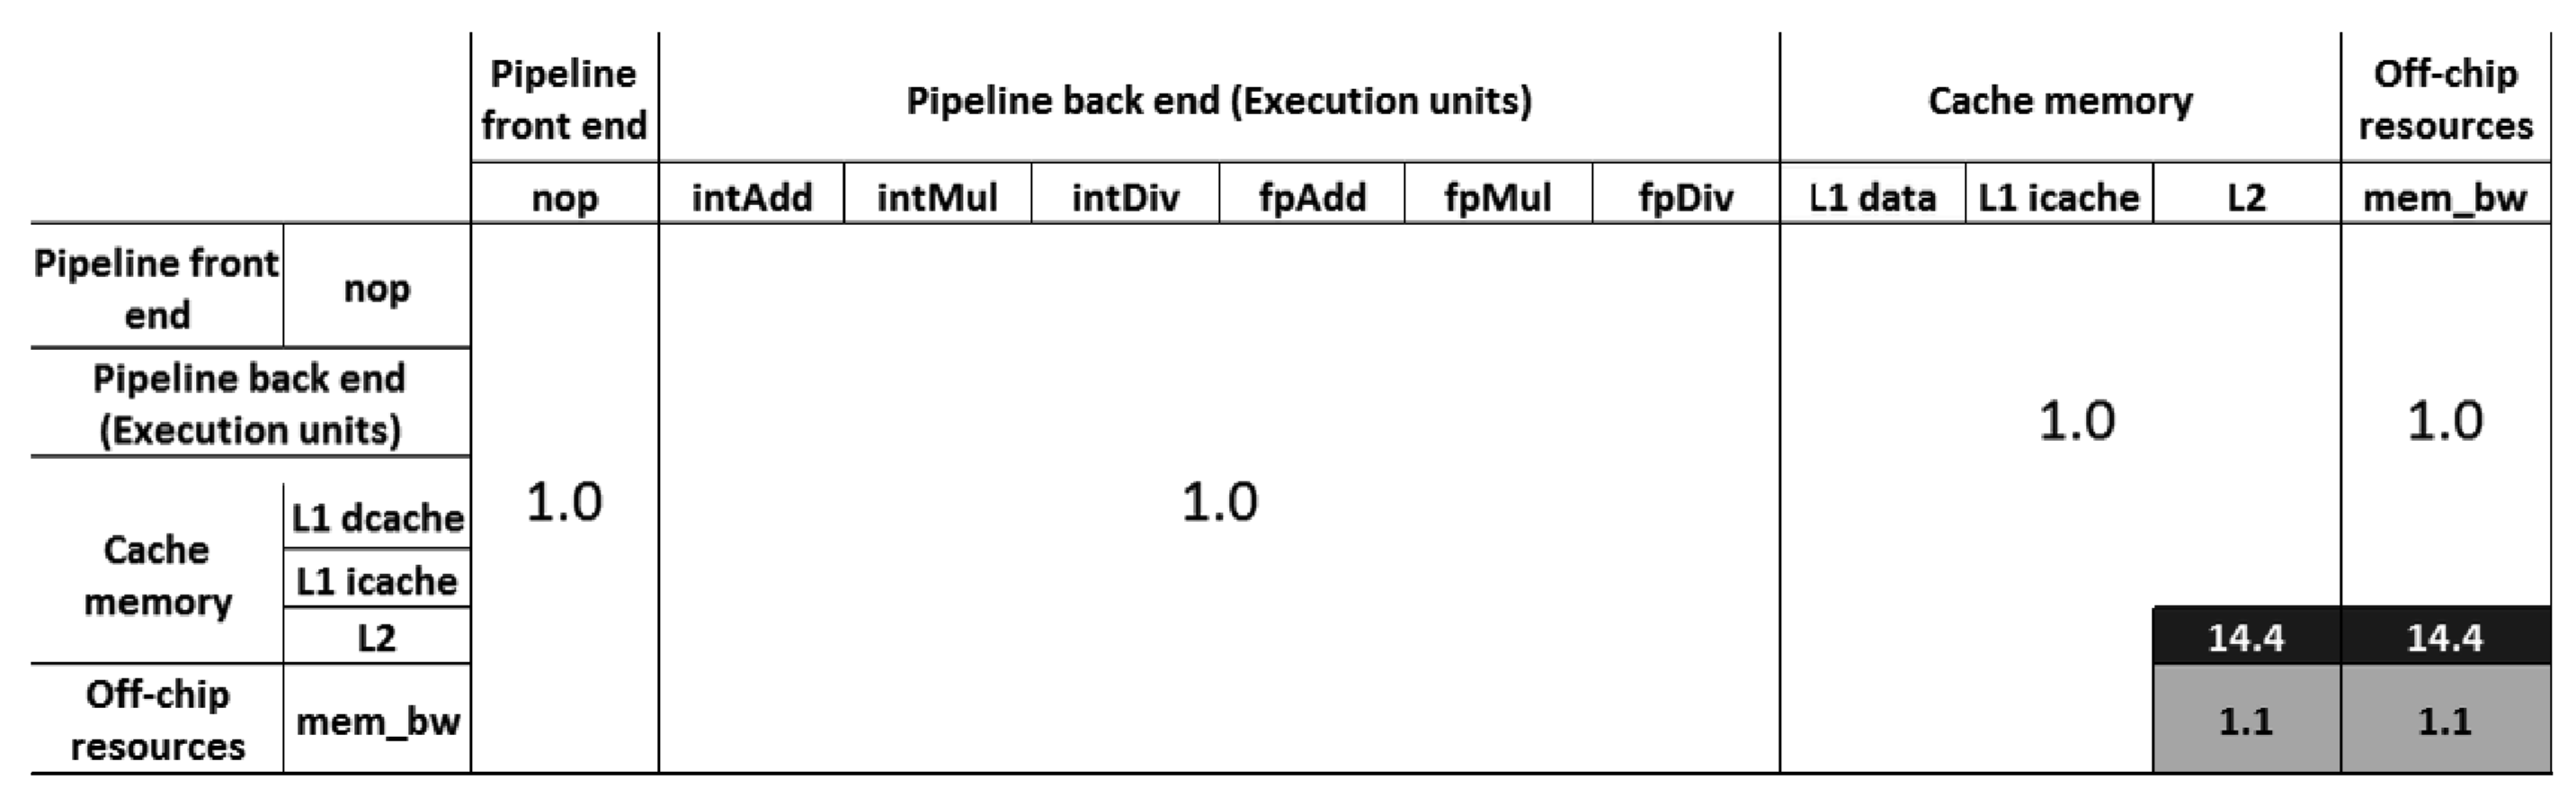
\includegraphics[width=\textwidth]{\chapterdirectory/figure/micro_bench/shared_cache_interference_detect.png}
\end{center}
\caption{Slowdown factor on the Intel Core2Quad within the same cluster (taken
from \cite{10.1145/2086696.2086713})}%
\label{fig:micro_bench:core2quad_stress}
\end{figure}

The application on a multi-core processor, however, is not as informative:
Figure~\ref{fig:micro_bench:core2quad_stress} shows the same experiment
performed within a cluster of an Intel Core2Quad (two separate cores that share
the same L2 cache, see Figure~\ref{fig:micro_bench:core2quad}). The results
indicate no unexpected slowdowns from the simultaneous use of components.
Information on slowdown due to simultaneous use of caches points is still
relevant and points to running two parallel cache intensive programs being
slower than one after the other.

\begin{figure}[hbt!]
\begin{center}
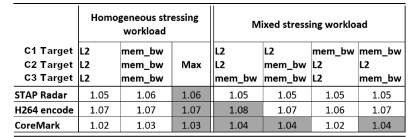
\includegraphics[width=0.5\textwidth]{\chapterdirectory/figure/micro_bench/simultaneous_stressing.png}
\end{center}
\caption{Standard benchmark interference on the Intel Core2Quad (taken
from \cite{10.1145/2086696.2086713})}%
\label{fig:micro_bench:core2quad_max_interference}
\end{figure}

\cite{10.1145/2086696.2086713} does not provide the analysis of potential
interference channels with more than two components in use simultaneously, but
it does analyze the slowdown factor suffered by some standard benchmark
applications running on one core when other components are being stressed by all
the other core.
The results are shown in
Figure~\ref{fig:micro_bench:core2quad_max_interference}. The observed slowdown
factors are very small, regardless of the components being stressed by the other
cores. This points to the use of standard benchmarks being poor indicators of
the worst slowdown that can be suffered because of interference. Indeed, none of
these results reflect the high slowdown factor that was obtained when even just
two cores stressed the same L2 cache. Thus, the effects of interference on an
application that uses the L2 cache more than those standard benchmarks is likely
to be much higher than what the results from
Figure~\ref{fig:micro_bench:core2quad_max_interference} would lead to believe.

\iffalse % Let's ignore the paper's actual contribution, shall we?
Figure~\ref{fig:micro_bench:atom_stress} shows the slowdown factors obtained by
this strategy on a Intel Atom Z530, which features a single core capable of
running two parallel threads. The lines correspond to the benchmark being
measured, the columns correspond to the target of the benchmark being used as
a source of interference.

The paper presents the same table for two other architectures: an Intel Pentium
D, with two cores each capable of a single thread; and an Intel Core2Quad
Q9550, with four cores, also only capable of a single thread. The resulting
slowdown factors for this particular set of shared resources for these two
architectures is considerably less impressive however, as only at most
two of these resources are actually shared by the separate cores (\textit{L2
cache}, and main memory access - \textit{mem\_bw}). Nevertheless, performing
such measurements does confirm that the resources are indeed not shared and
thus unable to interfere with one another, and the results do point out
L2 cache accesses to be a bottleneck on the Core2Quad architecture, with a
slowdown factor of $14.4$.

The results shown in \cite{10.1145/2086696.2086713}, especially those in
Figure~\ref{fig:micro_bench:atom_stress}, do make a strong argument against the
use of simultaneous multi-threading on a single core in applications with
real-time constraints, as having to taking into account the slowdown factor of
each of these shared resources makes the estimation of a precise worst-case
execution time that much more difficult. Unsurprisingly, such results are the
reason for simultaneous multi-threading being forbidden in aeronautical
contexts.
\fi

To summarize, the strategy employed here forms the basis of covert interference
channel identification, as it exposes potentially unknown links between
components, but it also provides some quantification of the architecture's
capabilities through the slowdown factor, and argues for the use of
micro-stressing benchmarks over that of standard ones for a true observation of
the maximum impact of interference, including for interference related to the
use of caches.

The next paper expands on this approach, by using performance monitors to
measure more than cycle counts, and thus learn more about how components
interact.

\stopallthesefloats

\stopallthesefloats{}
\subsection{Architecture and Application Characterization}
\begin{figure}
\begin{center}
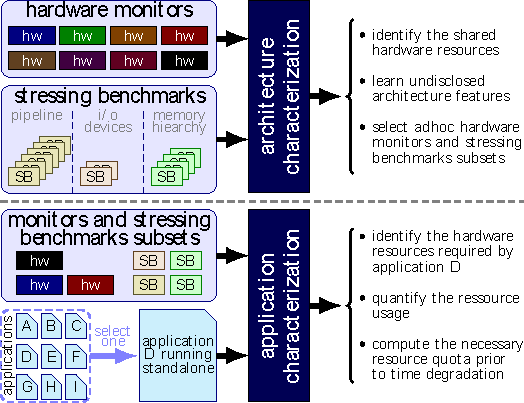
\includegraphics[width=0.7\textwidth]{\chapterdirectory/figure/micro_bench/co_running_apps_cots.pdf}
\end{center}
\caption{Strategy overview for \cite{Bin14} (Figure taken from the paper)}%
\label{fig:micro_bench:co_running_apps_cots}
\end{figure}

The approach presented in \cite{Bin14} can be seen as a follow up to the one of
\cite{10.1145/2086696.2086713}: the correlations between components that were
exposed are used to tailor the benchmarks performed on the application.  The
process is summarized in Figure~\ref{fig:micro_bench:co_running_apps_cots}.

When profiling the architecture, the objective is to characterize the hardware
itself, in order to identify shared hardware resources (including some that may
be missing from the architecture's documentation), determine their behavior when
in contention, potentially uncover unsuspected interactions between hardware
components, measure pertinent execution times and maximum bandwidths. To do so, the
approach starts with a comparison of each benchmark running in isolation and
running with other copies of itself running in parallel, as in the approach from
Section~\ref{sec:radojkovic} (the top-left diagonal in
Figure~\ref{fig:micro_bench:atom_stress}). In a second step, benchmarks
targeting different features are launched together. This provides information on
which parallel resource accesses affect one another. Here also, the approach is
similar to the one in Section~\ref{sec:radojkovic} (all cases other than the
top-left diagonal in Figure~\ref{fig:micro_bench:atom_stress}). Note that this
similarity with the previous section is to be expected, as both approaches make
similar assumptions on the availability of standard monitoring resources.  The
main difference being the use of hardware monitors other than the cycle counter
in \cite{Bin14}, where performance counters such as ``number of L1 hits'' are
also used in order to obtain a clearer understanding of the architecture, and
thus of the causes of the interference instead of just observing its effects.
This can be used to uncover relations between components despite not having
measured a change of slowdown factor upon their concurrent benchmarking.

Hardware monitors are counters that can be set to increase on the occurrence of
a given event, such as an access to the interconnect, a cache miss, a cache
eviction, and many other. The architecture's documentation generally provides a
list of events that can be monitored. These monitors can be reset, temporarily
frozen, or set to track another type of event during the execution of programs,
making them a very useful debugging and analysis tool.

\cite{Bin14} proposes using this information to limit the analysis made on
programs to what is truly necessary. Indeed, the architecture characterization
phase having already determined which combinations of benchmarks are redundant
for the analysis of interference between tasks, only a subset needs to be
employed to fully understand the impact of resource sharing on the
timing of the applications.

This subset of benchmark combinations is then used to analyze how much usage of
a particular resource is needed before an application slows down. In effect,
this indicates the minimal share of each resource needed for an application to
not suffer drastic worst case execution time slowdowns, and thus helps effective
scheduling of applications on a multi-core processor.

\begin{figure}[hbt!]
\begin{tabular}{cc}
\begin{subfigure}[t]{0.37\textwidth}
\lstinputlisting{\chapterdirectory/figure/micro_bench/paris_thesis_actual_general.txt}
\caption{Performance Counter Management}
\label{fig:micro_bench:co_running_apps_cots_algo_part_one}
\end{subfigure}
&
\begin{subfigure}[t]{0.47\textwidth}
\lstinputlisting{\chapterdirectory/figure/micro_bench/paris_thesis_general.txt}
\caption{Benchmark execution}
\label{fig:micro_bench:co_running_apps_cots_algo_part_deux}
\end{subfigure}
\end{tabular}
\caption{%
Benchmark algorithm used in \cite{Bin14} (extracted from \cite{Bin14Thesis})
}
\label{fig:micro_bench:co_running_apps_cots_algo}
\end{figure}

While \cite{Bin14} does not provide any code extracts, the algorithm can be
found in the associated thesis (\cite{Bin14Thesis}).
Figure~\ref{fig:micro_bench:co_running_apps_cots_algo} shows an overview of
algorithm used by \cite{Bin14}.
Figure~\ref{fig:micro_bench:co_running_apps_cots_algo_part_one} indicates how
the performance monitors are handled. The use of a loop to perform multiple
measures of the same experiment allow capture of the result's variability.
The benchmarked operations take the form shown in
Figure~\ref{fig:micro_bench:co_running_apps_cots_algo_part_deux}: it features an
unrolled loop (with \lstinline!UNROLLED! corresponding to the size of that inner
loop) within another loop, all performing the same operation (writing or
reading). The only reason for there to be an unrolled loop within the primary
loop is to reduce the amount of computations made during the iteration: the
combination of both loops simply makes the operations be performed across
the whole \lstinline!TABLESIZE! addresses. The \lstinline!STRIDE! parameter
corresponds to the gap between accesses, which is there to control the number of
times the same cache line is accessed. \cite{Bin14Thesis} indicates that the
use of the \lstinline!NOP! parameter is there to have idle time between
accesses: it corresponds to a varying number of \lstinline!nop! operations, and
can thus be used to see the effect of temporally spacing out the accesses.

The cache coherence identification part of this thesis
(Chapter~\ref{cha:identifying_cache_coherence}) uses an algorithm similar to the
one shown in Figure~\ref{fig:micro_bench:co_running_apps_cots_algo_part_one} to
observe the behavior of caches. In effect,
Chapter~\ref{cha:identifying_cache_coherence} is a specialized part of the
\textit{learn undisclosed architecture features} section of the
\textit{architecture characterization} process shown in
Figure~\ref{fig:micro_bench:co_running_apps_cots}. Instead of simply detecting
interaction It goes beyond the analysis
of simple interactions to really understand
\stopallthesefloats{}

\stopallthesefloats{}
\section{Analyzing Cache Performance}
The previous section showed approaches to the detection of potential
interference channels that could be applied to any component, but whose
genericity ran the risk of failing to detect complicated relations between
components. This section focuses on approaches that use benchmarks to
characterize cache coherence performance and/or interference channels.
\stopallthesefloats{}
\stopallthesefloats
\subsection{Cost of Cache Coherence}
\cite{Nowotsch2012LeveragingMC} places itself in a context similar to this
thesis: the issues of interference in multi-core architecture preventing their
use in avionics. More precisely, the paper proposes an analysis of an
architecture through benchmarks to ensure that tasks running in parallel can
correctly be time partitioned. The tasks in question involve mixed-criticality,
meaning that some tasks are more important than others, and thus lower
importance tasks must not impede higher importance ones.

The studied architecture is a NXP QorIQ P4080, featuring eight single-thread
cores with their own L1 and L2 caches, and interconnected through a CoreNet
Fabric implementing the MESI cache coherence protocol. There are also two L3
caches accessible through the interconnect.

The main sources of interference studied in \cite{Nowotsch2012LeveragingMC} are
simultaneous accesses to the interconnect and the main memory, as well as the
latencies induced by cache coherence. The idea is to have one core act as the
active observer, meaning that it is where time is measured, but it also performs
some operation. The other cores only act as a source of interference, and
multiple benchmarks are performed to see how increasing the number of secondary
cores influences the time measured by the observer core. This is similar to the
approaches presented in the previous section, with the difference being that
instead of targetting a specific component, the benchmarks are solely focused on
memory access, and the comparison is made on cores performing either
\textit{read} or \textit{write} on memory elements.

For the evaluation of the latencies induced by cache coherence, three categories
of cache coherence benchmarks are considered:
\begin{itemize}
\item \textbf{disabled:} No cache coherence enabled (i.e.~the baseline), where
its mechanisms are disabled and the cores do not target any of the same memory
elements.
\item \textbf{static:} Cache coherence mechanisms are enabled, but the cores
still do not target any of the same memory elements.
\item \textbf{dynamic:} Cache coherence enabled, and cores only target shared
memory elements.
\end{itemize}
This is made possible by the fact that the architecture supports disabling cache
coherence all together. For all three categories, sub-benchmarks are performed,
in which the observer core either reads or writes memory elements while the
secondary core also perform either reading or writing (thus resulting in four
combinations for each category of cache coherence: read read - \textit{rr}, read
- write, \textit{rw}, \textit{wr}, and \textit{ww}).

\begin{figure}[hbt!]
\lstinputlisting{\chapterdirectory/figure/micro_bench/06214768_code.txt}
\caption{%
Algorithm overview for \cite{Nowotsch2012LeveragingMC} (taken from the paper)
}
\label{fig:micro_bench:cache_coherence_avionics_algo}
\end{figure}

Figure~\ref{fig:micro_bench:cache_coherence_avionics_algo} shows the algorithm
used by \cite{10.1109/PACT.2009.22}. Prior to each measurement, the caches are
flushed, then the cores synchronize with each other. Time is recorder using
utilities from the cores, which avoids making \lstinline!time()! be a source of
interference. The measured operation takes three parameters:
\lstinline!OPERATION! corresponds to either reading or writing,
\lstinline!NBYTES! is the number of bytes accessed in a measurement,
\lstinline!GAP! is the distance between the accesses made in order to target
separate cache lines and thus ensure that all accesses are cache misses. The
number of measures is controlled by \lstinline!NMEAS!. The
\lstinline!__asm_write_loop_gap64! corresponds to a \lstinline!meas_loop! for
a writing operation with a gap of 64 bytes.

\begin{figure}[hbt!]
\begin{center}
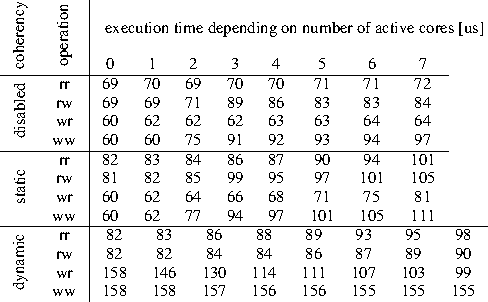
\includegraphics[width=0.7\textwidth]{\chapterdirectory/figure/micro_bench/cache_coherence_avionics.pdf}
\end{center}
\caption{Observed execution times depending on cache coherence and number of
active cores (adapted from \cite{Nowotsch2012LeveragingMC})}%
\label{fig:micro_bench:cache_coherence_avionics}
\end{figure}

The results of these benchmarks are shown in
Figure~\ref{fig:micro_bench:cache_coherence_avionics}.
\paragraph{Comparing \textit{Disabled} and \textit{Static} Cache Coherence:}
\textit{Static} cache coherence (mechanisms enabled, but each core access
different memory elements) does have an overhead compared to no cache
coherence at all when performing read operations, regardless of the operation
being performed by the other cores. For writing, this overhead is much lower.
This is interesting, as the \textit{static} benchmarks are the same experiment
as the \textit{disabled} cache coherence, meaning that effectively measures the
minimal overhead induced by having cache coherence mechanisms active,
regardless of how their are used. Thus, even when not having any use for it,
keeping cache coherence mechanisms enabled does lead to a increase in execution times.
This makes an argument for taking extra steps and disabling cache coherence for
memory elements that are not shared.

\paragraph{Comparing \textit{Static} and \textit{Dynamic} Cache Coherence:}
\textit{Dynamic} cache coherence (cache coherence enabled, and accesses
made to only shared memory elements) leads to the reverse: read operations yield
better execution time compared to writes. The best execution times are obtained by reading
while the other cores write, and the worst by writing while other cores are
writing as well. This is a surprising result (\textit{wr} and \textit{ww} being
slower than \textit{rr} and \textit{rw}), but these benchmarks do not take
coherence state of memory elements into account. The order in which cores get to
perform their operation changes that coherence state, and thus it changes the
cache's response  to other cores' operations, which in turn changes the execution time
results. Because of this, the results for \textit{dynamic} cache coherence
analysis cannot be exploited for a precise measurement of the effects of cache
coherence on running software.

To summarize, \cite{Nowotsch2012LeveragingMC} does provide an interesting
metric, which is found by comparing the execution time between the \textit{disabled}
and \textit{static} benchmarks. The overhead caused by unrequited cache
coherence queries are considered to be a form of interference.  Indeed, this
corresponds to the \textit{minor} interference of
Chapter~\ref{chap:exposing_interference} (see
Definition~\ref{def:interference:minor}).

The lack of information on coherence states prevent the \textit{dynamic}
benchmarks from being reused in the context of this thesis. However, a more
appropriate form of benchmarking for cache coherence mechanisms with shared
memory elements is explored in the next section.

\stopallthesefloats

\stopallthesefloats{}
\subsection{Cache Performance Analysis}
\label{sec:nehalem}

\begin{figure}[hbt!]
\centering
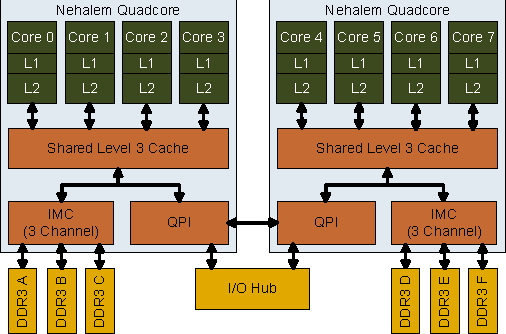
\includegraphics[width=0.6\columnwidth]{\chapterdirectory/figure/micro_bench/intel_nehalem.pdf}
\caption{%
Interconnected Intel Nehalem processors (extracted from \cite{10.1109/PACT.2009.22}).
}
\label{fig:micro_bench:intel_nehalem}
\end{figure}

\cite{10.1109/PACT.2009.22} is a paper on benchmarks performed on the Intel
Nehalem architecture (see Figure~\ref{fig:micro_bench:intel_nehalem}), which
uses the MESIF cache coherence protocol and has an inclusive cache hierarchy.
For clarification's sake, the cache coherence protocol is active below the L3
cache, meaning that this dual processor architecture effectively results in
only two caches being made coherent through MESIF.

To perform the benchmarks comparing the effect of coherence states of memory
element on writing and reading performance, their benchmark library makes it so
they are able to put data in the desired stable coherence state in the cache
they want, potentially using the other processor to attain the desired state.
In effect, this allows control of the coherence states of the system prior to
the start of the benchmark.  To reach the desired state in the caches of core
$N$, the following strategy is employed:
\begin{description}
\item[Modified] Core $N$ writes the data.
\item[Exclusive] Core $N$ writes the data (thus invalidating the other cores'
data), flushes, then reads the data.
\item[Shared] Core $N$ reaches the \textit{Exclusive} state, then another core
reads the same data.
\end{description}

There is an interesting omission: the \textit{Forward} state is not considered.
The authors indicate expecting the \textit{Forward} state to only become an
improvement for systems in which there are more than two processors and is thus
assumed not to have any effect on the benchmarks of their dual processor
architecture. This is incorrect, but, as explained later, the effects of the
\textit{Forward} are not seen in their results, since the benchmarks which would
have been affected were also omitted.

On the other hand, the strategy to reach a selected state for core $N$ described
above is still valid, even when ignoring the \textit{Forward}. Indeed, with this
process, the \textit{Forward} state only appears when reaching the
\textit{Shared} state, but it is reached by the core that ``reads the same
data'', not core $N$. In reality, having a \textit{Forward} state in an
architecture with only two caches does actually have some benefits: if the two
caches have read certain data, then one wants to write to it. Without
\textit{Forward} state, the cache wanting to write will have to fetch data in
RAM, whereas with the \textit{Forward} state available, it might be provided by
the other cache or simply ot have to fetch it in RAM (depending on which cache
performed a write first, and choices of implementation). Similarly, it has an
impact if a cache line is read by both caches, but the cache not in the
\textit{Forward} cache evicts it at some point, them re-acquires it. This would
have had an observable result when measuring the writing execution time. Indeed,
writing when core $N$ is in the \textit{Shared} state and another core is in the
\textit{Forward} state should result in faster execution time than when the other core
is in the \textit{Shared} state. Since The paper does not feature a table
proving a list of execution time when writing, but only for benchmarks that reading,
this difference cannot be seen and one might erroneously assume that the
\textit{Forward} state does indeed have no impact on systems with coherence
maintained between only two caches.

\iffalse
Considerations are taken to minimize any mechanic interfering with the
benchmarks: transaction look-aside buffers are pre-loaded and accessed memory
elements are not adjacent to avoid any pre-fetching optimization.
\fi

\begin{figure}[hbt!]
\begin{tabular}{cc}
\begin{subfigure}[t]{0.47\textwidth}
\lstinputlisting{\chapterdirectory/figure/micro_bench/algo_nehalem_latency.txt}
\caption{Latency benchmarks}
\label{fig:micro_bench:intel_nehalem_latency_algo}
\end{subfigure}
&
\begin{subfigure}[t]{0.47\textwidth}
\lstinputlisting{\chapterdirectory/figure/micro_bench/algo_nehalem_bandwidth.txt}
\caption{Bandwidth benchmarks}
\label{fig:micro_bench:intel_nehalem_bandwidth_algo}
\end{subfigure}
\end{tabular}
\caption{%
Algorithm overview for \cite{10.1109/PACT.2009.22} (taken from the paper)
}
\label{fig:micro_bench:intel_nehalem_algo}
\end{figure}

Figure~\ref{fig:micro_bench:intel_nehalem_latency_algo} shows an overview of the
algorithm used by \cite{10.1109/PACT.2009.22} to measure execution times. The steps
described are more about what is done prior to the measurements themselves.
Warming up the transaction look-aside buffer means pre-loading all entries in
order to avoid this loading being taken into account in the resulting execution time.
The accesses made for the measured part of the benchmark correspond to a pointer
chasing algorithm, just like in \cite{10.1145/2086696.2086713} (see
Figure~\ref{fig:micro_bench:co_running_apps_cots_algo_part_deux}).

The bandwidth benchmarking algorithm is shown in
Figure~\ref{fig:micro_bench:intel_nehalem_bandwidth_algo}. Synchronization
between the threads is more thoroughly controlled in this one: by memorizing the
exact window upon which each thread made its accesses, the window corresponding
to the period in which all threads were performing accesses can be obtained.
The bandwidth can then be obtained from the number of accesses successfully
performed within this window.

\begin{figure}[hbt!]
\centering
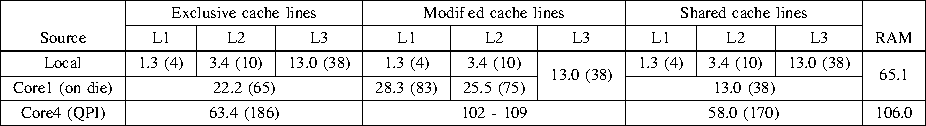
\includegraphics[width=\textwidth]{\chapterdirectory/figure/micro_bench/nehalem_read_latencies.pdf}
\caption{%
Latencies of reading from Core 0, results in ``nanoseconds (cycles)'' (Figure
taken from \cite{10.1109/PACT.2009.22})
}
\label{fig:micro_bench:intel_nehalem_read_latencies}
\end{figure}

Figure~\ref{fig:micro_bench:intel_nehalem_read_latencies} shows the results of
benchmarks measuring the time required for the core 0 to read data held in
various locations, according to the state of the data in the remote location.
Unsurprisingly, accesses made to the local L1 and L2 caches was not impacted by
the state of the data in the L3 cache. It appears this also holds true for the
local L3 cache itself. Access to data held in the caches of another core on the
same processor does vary depending on the coherence state. According to
\cite{10.1109/PACT.2009.22}, this is explained by the L3 cache having to check
on the L2 and L1 caches of that other core, as, unless the state is
\textit{Shared}, the L1 and L2 cores may hold a more up-to-date value. For data
held in the other processor, the results are as expected, with the cost of
traversing the bridge between both processors being added when accessing memory
elements in either the \textit{Exclusive} or \textit{Shared} state, but also
having a higher cost when accessing \textit{Modified} memory elements: as
explained in \cite{10.1109/PACT.2009.22} and Chapter~\ref{cha:cache_coherence},
\textit{Modified} memory elements are wrote back to the memory prior to being
sent as a reaction to a \textit{GetS} query.

\begin{figure}[hbt!]
\centering
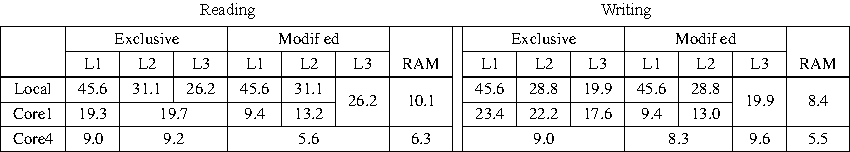
\includegraphics[width=\textwidth]{\chapterdirectory/figure/micro_bench/nehalem_bandwidths.pdf}
\caption{%
Bandwidth for access from Core 0, results in GB/s (Figure
taken from \cite{10.1109/PACT.2009.22})
}
\label{fig:micro_bench:intel_nehalem_broad}
\end{figure}

\cite{10.1109/PACT.2009.22} does however perform more analyses on the
performance of cache accesses. The second half of the paper is dedicated to
bandwidth analysis, of which the results are shown in
Figure~\ref{fig:micro_bench:intel_nehalem_broad}. These results are coherent
with their equivalent in the execution time benchmarks. They do provide more
information than what was available in the documentation however, such as actual
maximum bandwidth instead the theoretical maximal one.

The approach presented in \cite{10.1109/PACT.2009.22} is a good solution for the
\textit{benchmark} part of the framework described in
Section~\ref{sec:second_intro:framework}. Indeed, by taking into account the
coherence state of the targeted memory elements, \cite{10.1109/PACT.2009.22}
ensures the system state that led to the recording of the execution time is
understood and thus, that the correct execution time will be expected when attempting
to predict the architecture's behavior.
\stopallthesefloats

\stopallthesefloats{}
\section{Finding Elusive Hardware Monitors}
\label{sec:elusive_hardware_monitors}
\begin{figure}[hbt!]
\centering
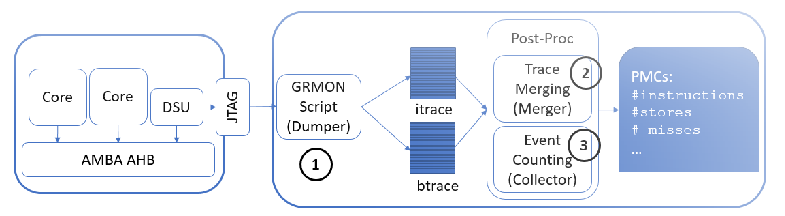
\includegraphics[width=\columnwidth]{\chapterdirectory/figure/micro_bench/expose_monitor_general_approach.pdf}
\caption{%
Trace collection process (extracted from \cite{palomo_et_al:LIPIcs:2020:12378})
}
\label{fig:micro_bench:expose_monitors}
\end{figure}

\cite{palomo_et_al:LIPIcs:2020:12378} presents a case study for the profiling of
architectures where performance monitors are not available. This is interesting,
because architecture profiling usually assumes that they are available. Having
a way to profile architectures without would extend the range of architectures
that can be considered for critical real-time contexts.

The architecture being studied in \cite{palomo_et_al:LIPIcs:2020:12378} is
system-on-chip with a dual-core processor.  While it does not have performance
monitors, it does have some hardware debugging features, which can be accessed
using a \textit{JTAG} port.

These hardware debugging features can snoop the messages passing through the
interconnect, as well as the instructions executed by each core (and their
program counter). In the approach proposed by
\cite{palomo_et_al:LIPIcs:2020:12378}, the platform is configured so that these
two sources of information are stored into circular buffers (within the chip).
The \textit{JTAG} connection is used to continuously copy these buffers into an
external analysis platform (see Figure~\ref{fig:micro_bench:expose_monitors}).
The speed at which these buffers are filled is higher than that of the
\textit{JTAG} connection, meaning that information would be lost if the programs
were running normally. Thus, the \textit{GRMON} script takes control of the
execution once the section of the programs under analysis is reached, and
proceeds to running the applications in a \textit{step-by-step} manner, which
ensures no information is lost.

Once this event capture is completed, the post-processing steps begin, starting
with a clean-up phase (\textit{Trace Merging}), which clears out redundant data.
Then comes the \textit{Event Counting} phase, which matches instructions to bus
events in order to recognize patterns that fit known events. For example, data
cache load misses are identified by seeing a load instruction be performed by
a core one cycle \textit{after} seeing the matching query go through the
interconnect.

Thus, instead of relying on performance counters, it is possible to obtain an
accurate description of the behavior of the platform through capture and
analysis of execution traces. Such strategies extend the range of platforms upon
which profiling is possible, including for the purpose of identifying cache
coherence using the process described in
Chapter~\ref{cha:identifying_cache_coherence}.

\stopallthesefloats{}
\section{Conclusion}
The approach shown in Section~\ref{sec:nehalem} is adequate for the second step
of the framework presented in this thesis (see
Section~\ref{sec:second_intro:framework}), in which the performance of the
architecture's cache coherence mechanisms are measured in order to feed them to
a model. Indeed, it does provide interesting information about single
instruction execution time according to the type of instruction being performed
(\loadinstr{} or \storeinstr{}) and the cache coherence state. It does not,
however, attempt to analyze the internals of the cache coherence mechanisms used
by the architecture. In fact, some of them are explicitly ignored
(\textit{Forward} state). Thus, while being an important step, it remains
insufficient to provide the user with enough information to understand what
interference could be generated by cache coherence mechanisms, unless the
identification step proposed in this thesis is applied.

Furthermore, approaches such as the one described in
Section~\ref{sec:elusive_hardware_monitors} can be used to apply the framework
presented in this thesis to architectures with more restricted monitoring
facilities.
